%TODO da modificare con la One Time Password. Aggiungere UC per invio dati da parte dell'admin all'utente. da aggiungere UC-1.4 per inserimento password temporanea da parte dell'amministratore.
%TODO mettere prima login utente, poi rifare tutti gli indici.
\subsection{UC-4 Recupero password}
\begin{itemize}
	\item \textbf{Attore primario:} utente non autenticato;

	\item \textbf{Descrizione:} l'utente è già registrato e non si ricorda la sua attuale password e desidera cambiarla;

	\item \textbf{Precondizioni:} l'utente è già registrato presso il sistema e ha cliccato il link per l'impostazione di una nuova password tramite schermata di login;

	\item \textbf{Postcondizioni:} l'utente ha cambiato la propria password con successo;

	\item \textbf{Scenario principale:}
	      \begin{enumerate}
	      	      \item l'utente inserisce la propria mail di registrazione per il recupero della password (UC-4.1 Inserimento email di registrazione per il recupero password);
		      \item il sistema invia una mail all'indirizzo email inserito precedentemente se l'indirizzo email è censito all'interno del sistema, in caso contrario verrà segnalato un errore a video e non verrà inviato alcun link alla mail inserita precedentemente (UC-5 Visualizzazione errore relativo ad una mail non presente all'interno del sistema nel recupero password);
		      \item l'utente inserisce la nuova password all'interno del campo dati della pagina aperta tramite link (UC-4.2 Inserimento di una nuova password nell'operazione di recupero password);
		      \item l'utente conferma con successo la password inserita (UC-4.3 Conferma della password inserita);
		      \item il sistema restituisce un messaggio comunicante l'avvenuto cambiamento della password.
	      \end{enumerate}
\end{itemize}

%TODO cambiare l'immagine
\begin{figure}[H]
	\centering
	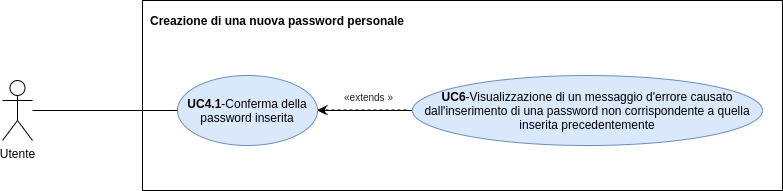
\includegraphics[width=\textwidth]{src/CasiDUso/immagini/SottocasoCreazionePassword.png}
	\caption{Zoom-in creazione password.}
\end{figure}

\subsubsection{UC-4.1 Inserimento email di registrazione per il recupero password}
\begin{itemize}
	\item \textbf{Attore primario:} utente non autenticato;

	\item \textbf{Descrizione:} l'utente vuole inserire il proprio indirizzo email su cui farsi mandare il link di recupero password;

	\item \textbf{Precondizioni:} l'utente ha cliccato sul link per la reimpostazione della password;

	\item \textbf{Postcondizioni:} l'utente ha inserito con successo la propria mail di registrazione;

	\item \textbf{Scenario principale:}
	      \begin{enumerate}
		      \item l'utente seleziona il campo dati in cui inserire la propria mail di registrazione;
		      \item l'utente inserisce la propria mail di registrazione;
		      \item l'utente invia i dati al sistema;
		      \item il sistema controlla la presenza dell'indirizzo email all'interno del database e, qualora fosse presente, invierà il link di recupero password;
	      \end{enumerate}
	\item \textbf{Estensioni:}
	      \begin{enumerate}
		      \item UC-6 visualizzazione di un messaggio d'errore causato dall'inserimento di una mail non valida.
	      \end{enumerate}
\end{itemize}

%TODO da valutare se sdoppiarlo nel caso in cui l'utente non sia autenticato e voglia recuperare la password e nel caso in cui voglia modificare la password da autenticato.
\subsubsection{UC-4.3 Conferma della password inserita}
\begin{itemize}
	\item \textbf{Attore primario:} utente;

	\item \textbf{Descrizione:} l'utente vuole confermare la password inserita;

	\item \textbf{Precondizioni:} l'utente ha inserito una nuova password valida all'interno della pagina per l'inserimento di una nuova password;

	\item \textbf{Postcondizioni:} l'utente ha inserito con successo la stessa password inserita precedentemente;

	\item \textbf{Scenario principale:}
	      \begin{enumerate}
		      \item l'utente inserisce la password precedentemente inserita;
		      \item il sistema analizza il matching tra le due password e in caso di errore restituisce un messaggio d'errore esplicativo e richiede nuovamente l'inserimento di una nuova password senza precedentemente completare la modifica della password.
	      \end{enumerate}
	\item \textbf{Estensioni:}
	      \begin{enumerate}
		      \item UC-6 Visualizzazione di un messaggio d'errore causato dall'inserimento di una password non corrispondente a quella inserita precedentemente.
	      \end{enumerate}
\end{itemize}

%TODO attore sistema? sdoppiare anche questo UC come discusso sopra?
\subsection{UC-5 Visualizzazione di un errore in seguito all'inserimento di una password non valida}
\begin{itemize}
	\item \textbf{Attore primario:} utente;

	\item \textbf{Descrizione:} viene visualizzato un messaggio d'errore a seguito dell'inserimento di una password non valida da parte di un utente durante l'impostazione di una nuova password;

	\item \textbf{Precondizioni:} l'utente ha inserito una password non valida durante l'impostazione di una nuova password.

	\item \textbf{Postcondizioni:} il sistema restituisce un messaggio d'errore esplicativo e chiede all'utente di inserire una nuova password valida senza apportare le modifiche;

	\item \textbf{Scenario principale:}
	      \begin{enumerate}
		      \item il sistema elabora la richiesta ricevuta;
		      \item il sistema restituisce un messaggio d'errore esplicativo che viene visualizzato sullo schermo del dispositivo dell'utente e non completa la registrazione del nuovo utente fino a quando non viene inserita una password corretta.
	      \end{enumerate}
\end{itemize}

%TODO idem a sopra
\subsection{UC-6 Visualizzazione di un messaggio d'errore causato dall'inserimento di una password non corrispondente a quella inserita precedentemente}
\begin{itemize}
	\item \textbf{Attore primario:} utente;

	\item\textbf{Descrizione:} l'utente vuole confermare la password inserita. Viene visualizzato un messaggio d'errore causato dall'inserimento di una password di conferma errata;

	\item\textbf{Precondizioni:} l'utente ha inserito una nuova password valida all'interno della pagina per l'inserimento di una nuova password e ha inserito una password di conferma diversa da quella inserita precedentemente;

	\item\textbf{Postcondizioni:} viene visualizzato un messaggio d'errore causato dall'inserimento di una password di conferma errata;

	\item \textbf{Scenario principale:}
	      \begin{enumerate}
		      \item l'utente inserisce la password precedentemente inserita;
		      \item il sistema analizza il matching tra le due password, in caso negativo restituisce un messaggio d'errore esplicativo e richiede nuovamente l'inserimento di una nuova password senza precedentemente completare la modifica della password.
	      \end{enumerate}
\end{itemize}

%TODO valutare se fare relativi UC per inserimento mail ed inserimento password.
\subsection{UC-7 Login tramite applicazione mobile}
\begin{itemize}
	\item \textbf{Attore primario:} utente non autenticato;

	\item \textbf{Descrizione:} l'utente vuole autenticarsi presso il sistema tramite l'inserimento del proprio indirizzo e-mail di registrazione e la propria password;

	\item \textbf{Precondizioni:} l'utente è registrato presso il sistema;

	\item \textbf{Postcondizioni:} l'utente è autenticato presso il sistema;

	\item\textbf{Scenario principale:}
	      \begin{enumerate}
		      \item l'utente avvia l'applicazione mobile;
		      \item l'utente seleziona la funzionalità "Accedi";
		      \item l'utente inserisce il proprio indirizzo e-mail con il quale si è registrato presso il sistema;
		      \item l'utente inserisce la propria password;
		      \item l'utente invia i dati al sistema;
		      \item il sistema elabora la richiesta e aggiorna la schermata del dispositivo con la dashboard personale qualora il login venga eseguito con successo. In caso contrario il sistema restituisce un messaggio d'errore esplicativo e non completa il login dell'utente.
	      \end{enumerate}
	\item \textbf{Estensioni:}
	      \begin{enumerate}
		      \item UC-9 Visualizzazione di un messaggio d'errore a causa di un login errato.
	      \end{enumerate}
\end{itemize}
